\documentclass[12pt,a4paper]{article}
\usepackage[utf8]{vietnam}
\usepackage{amsmath,amssymb}
\usepackage{tabularx}
\usepackage{tikz}
\usetikzlibrary{calc,angles,quotes,arrows.meta,patterns}
\usepackage{xcolor}
\usepackage{enumitem}
\usepackage{fancyhdr}
\usepackage{graphicx}
\usepackage[top=0.9cm, bottom=0.9cm, left=1.2cm, right=1.2cm]{geometry}
\usepackage[loigiai]{ex_test}
\SAOPTN{widthSA=3.2,heightSA=0.62}

\setlength{\headheight}{15pt}
\setlength{\parskip}{0pt}

\pagestyle{fancy}
\fancyhf{}
\rhead{\textit{Môn Toán 9 -- Hướng dẫn giải Đề số 03}}
\lhead{\textit{Bộ đề ôn tập Giữa học kì I}}
\cfoot{\thepage}

\begin{document}

\begin{center}
  \textbf{\Large HƯỚNG DẪN GIẢI CHI TIẾT VÀ BẢNG ĐÁP ÁN}\\
  \textbf{\large ĐỀ ÔN TẬP GIỮA HỌC KỲ I -- ĐỀ SỐ 03}\\
  \textit{Môn: Toán 9 -- Năm học 2026 -- 2027}
\end{center}
\vspace{2mm}

% --- BẢNG ĐÁP ÁN TRẮC NGHIỆM TÓM TẮT ---
\noindent\textbf{\large A. BẢNG ĐÁP ÁN TRẮC NGHIỆM TỔNG HỢP}
\vspace{1mm}

\noindent\textbf{1. Phần I (Mỗi câu trả lời đúng được 0,25 điểm):}
\begin{center}
\begin{tabular}{|c|c|c|c|c|c|c|c|c|c|c|c|c|}
\hline
\textbf{Câu} & \textbf{1} & \textbf{2} & \textbf{3} & \textbf{4} & \textbf{5} & \textbf{6} & \textbf{7} & \textbf{8} & \textbf{9} & \textbf{10} & \textbf{11} & \textbf{12} \\
\hline
\textbf{Đ/A} & \textbf{B} & \textbf{A} & \textbf{B} & \textbf{C} & \textbf{D} & \textbf{B} & \textbf{C} & \textbf{A} & \textbf{D} & \textbf{C} & \textbf{A} & \textbf{B} \\
\hline
\end{tabular}
\end{center}
\vspace{0.5mm}

\noindent\textbf{2. Phần II (Đúng 1 ý: 0,1đ; Đúng 2 ý: 0,25đ; Đúng 3 ý: 0,5đ; Đúng 4 ý: 1,0đ):}
\begin{center}
\begin{tabular}{|c|c|c|c|c||c|c|c|c|c|}
\hline
\textbf{Câu 1} & \textbf{a)} & \textbf{b)} & \textbf{c)} & \textbf{d)} & \textbf{Câu 2} & \textbf{a)} & \textbf{b)} & \textbf{c)} & \textbf{d)} \\
\hline
\textbf{Đáp án} & Đ & S & S & Đ & \textbf{Đáp án} & Đ & Đ & S & Đ \\
\hline
\end{tabular}
\end{center}
\vspace{0.5mm}

\noindent\textbf{3. Phần III (Mỗi câu trả lời đúng được 1,0 điểm):}
\begin{center}
\begin{tabular}{|c|c|c|}
\hline
\textbf{Câu} & \textbf{Câu 1} & \textbf{Câu 2} \\
\hline
\textbf{Đáp án} & Nam: 22, Nữ: 18 & $62^\circ$ \\
\hline
\end{tabular}
\end{center}
\vspace{2mm}

% --- LỜI GIẢI CHI TIẾT ---
\noindent\textbf{\large B. HƯỚNG DẪN GIẢI CHI TIẾT TỪNG CÂU}
\vspace{1mm}

\noindent\textbf{\large PHẦN I. CÂU TRẮC NGHIỆM NHIỀU PHƯƠNG ÁN LỰA CHỌN}
\vspace{1mm}
\begin{ex}
Phương trình nào sau đây là phương trình bậc nhất hai ẩn?
\choice
{$2x^2 - 3y = 1$}
{\True $x - 3y = 1$}
{$3x^2 + 2y = 1$}
{$0x + 0y = 1$}
\loigiai{
Phương trình bậc nhất hai ẩn có dạng tổng quát là $ax + by = c$, trong đó các hệ số $a, b$ không đồng thời bằng 0 và các ẩn đều có bậc 1. Do đó $x - 3y = 1$ là phương trình bậc nhất hai ẩn.
\par\textbf{Chọn đáp án B.}
}
\end{ex}

\begin{ex}
Phương trình nào dưới đây nhận cặp số $(-2; 4)$ làm nghiệm?
\choice
{\True $2x + y = 0$}
{$x - y = 1$}
{$x - 2y = 0$}
{$x + 2y + 1 = 0$}
\loigiai{
Thay $x = -2, y = 4$ vào phương trình $2x + y = 0$: $2(-2) + 4 = -4 + 4 = 0$ (thỏa mãn).
\par\textbf{Chọn đáp án A.}
}
\end{ex}

\begin{ex}
Phương trình $(x^2 + 9)(2x + 3) = 0$ có số nghiệm là:
\choice
{$0$}
{\True $1$}
{$2$}
{$3$}
\loigiai{
Vì $x^2 + 9 \ge 9 > 0$ với mọi số thực $x$ nên phương trình $x^2 + 9 = 0$ vô nghiệm. Do đó $(x^2 + 9)(2x + 3) = 0 \iff 2x + 3 = 0 \iff x = -\frac{3}{2}$. Vậy phương trình có đúng $1$ nghiệm.
\par\textbf{Chọn đáp án B.}
}
\end{ex}

\begin{ex}
Hệ phương trình nào sau đây có vô số nghiệm?
\choice
{$\begin{cases} 2x - 5y = 1 \\ -x + 3y = 2 \end{cases}$}
{$\begin{cases} 2x - 5y = 1 \\ x + 3y = 2 \end{cases}$}
{\True $\begin{cases} 2x - 5y = 1 \\ -x + \frac{5}{2}y = -\frac{1}{2} \end{cases}$}
{$\begin{cases} 2x - 5y = 1 \\ -x - 3y = 2 \end{cases}$}
\loigiai{
Nhân cả hai vế của phương trình thứ hai ở hệ C với $-2$, ta được phương trình $2x - 5y = 1$, trùng hoàn toàn với phương trình thứ nhất. Do đó hệ phương trình C có vô số nghiệm.
\par\textbf{Chọn đáp án C.}
}
\end{ex}

\begin{ex}
Nghiệm của hệ phương trình $\begin{cases} 4x = 8 \\ 3x + 2y = 10 \end{cases}$ là:
\choice
{$(1; 2)$}
{$(2; 3)$}
{$(3; 4)$}
{\True $(2; 2)$}
\loigiai{
Từ $4x = 8 \implies x = 2$. Thay vào phương trình thứ hai: $3(2) + 2y = 10 \iff 6 + 2y = 10 \iff 2y = 4 \iff y = 2$. Vậy nghiệm của hệ là $(2; 2)$.
\par\textbf{Chọn đáp án D.}
}
\end{ex}

\begin{ex}
Cho hệ phương trình $\begin{cases} 4x - y = 2 \\ x + 3y = 7. \end{cases}$ Cặp số nào dưới đây là nghiệm của hệ phương trình đã cho?
\choice
{$(2; 2)$}
{\True $(1; 2)$}
{$(-1; -2)$}
{$(2; -2)$}
\loigiai{
Thay cặp số $(1; 2)$ vào hệ: $4(1) - 2 = 2$ và $1 + 3(2) = 7$, cả hai phương trình đều thỏa mãn. Vậy cặp số $(1; 2)$ là nghiệm của hệ.
\par\textbf{Chọn đáp án B.}
}
\end{ex}

\begin{ex}
Trong các cặp số sau, cặp số nào là nghiệm của phương trình $x + y = 3$?
\choice
{$(8; 1)$}
{$(-3; 6)$}
{\True $(4; -1)$}
{$(0; 2)$}
\loigiai{
Thay $(4; -1)$ vào phương trình: $4 + (-1) = 3$ (thỏa mãn).
\par\textbf{Chọn đáp án C.}
}
\end{ex}

\begin{ex}
Cặp số $(x; y) = (3; -1)$ là nghiệm của hệ phương trình nào sau đây?
\choice
{\True $\begin{cases} 2x + y = 5 \\ 3x - 2y = 11 \end{cases}$}
{$\begin{cases} 2x + 2y = 5 \\ 3x - 2y = 11 \end{cases}$}
{$\begin{cases} 2x + y = 6 \\ 3x - 2y = 1 \end{cases}$}
{$\begin{cases} 2x + y = -6 \\ 3x + y = 10 \end{cases}$}
\loigiai{
Thay $x = 3, y = -1$ vào hệ phương trình A: $2(3) + (-1) = 5$ và $3(3) - 2(-1) = 9 + 2 = 11$ (đều thỏa mãn).
\par\textbf{Chọn đáp án A.}
}
\end{ex}

\begin{ex}
Cho tam giác $ABC$ vuông tại $A$. Khi đó tỉ số lượng giác $\tan B$ bằng:
\choice
{$\frac{AB}{BC}$}
{$\frac{AC}{BC}$}
{$\frac{CB}{BA}$}
{\True $\frac{AC}{AB}$}
\loigiai{
Trong tam giác $ABC$ vuông tại $A$, cạnh đối diện góc $B$ là $AC$, cạnh kề góc $B$ là $AB$. Do đó $\tan B = \frac{\text{cạnh đối}}{\text{cạnh kề}} = \frac{AC}{AB}$.
\par\textbf{Chọn đáp án D.}
}
\end{ex}

\begin{ex}
Cho tam giác $ABC$ vuông tại $A$, đường cao $AH \perp BC$ ($H \in BC$). Biết $AH = 6, BH = 3$. Giá trị $\sin B$ bằng:
\choice
{$\frac{\sqrt{3}}{3}$}
{$\frac{\sqrt{3}}{2}$}
{\True $\frac{2\sqrt{5}}{5}$}
{$\frac{\sqrt{3}}{6}$}
\loigiai{
Trong tam giác vuông $ABH$ tại $H$: $AB = \sqrt{AH^2 + BH^2} = \sqrt{6^2 + 3^2} = \sqrt{45} = 3\sqrt{5}$. Khi đó $\sin B = \frac{AH}{AB} = \frac{6}{3\sqrt{5}} = \frac{2}{\sqrt{5}} = \frac{2\sqrt{5}}{5}$.
\par\textbf{Chọn đáp án C.}
}
\end{ex}

\begin{ex}
Cho tam giác $ABC$ vuông tại $A$, đường cao $AH \perp BC$ ($H \in BC$). Biết $BH = 3, HC = 1$. Số đo góc $B$ là:
\choice
{\True $30^\circ$}
{$60^\circ$}
{$70^\circ$}
{$45^\circ$}
\loigiai{
Áp dụng hệ thức lượng: $AH^2 = BH \cdot HC = 3 \cdot 1 = 3 \implies AH = \sqrt{3}$. Trong tam giác vuông $ABH$ tại $H$: $\tan B = \frac{AH}{BH} = \frac{\sqrt{3}}{3} \implies \widehat{B} = 30^\circ$.
\par\textbf{Chọn đáp án A.}
}
\end{ex}

\begin{ex}
Cho hình vẽ tam giác vuông $ABH$ vuông tại $H$ với $BH = 10\text{ m}$ và $\widehat{B} = 60^\circ$. Chiều cao $AH$ có độ dài là:
\begin{center}
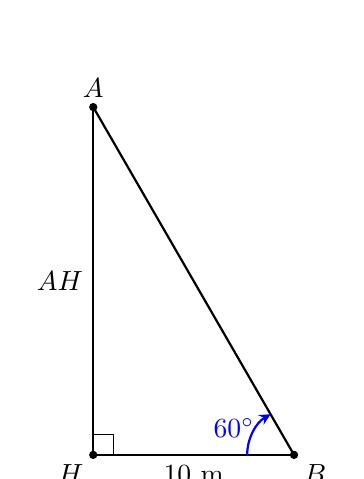
\begin{tikzpicture}[scale=0.85, line join=round, line cap=round, >=stealth]
  \coordinate (H) at (0,0);
  \coordinate (B) at (3,0);
  \coordinate (A) at (0,5.196); % 3 * sqrt(3)
  \draw[thick] (H) -- (B) node[midway, below] {$10\text{ m}$};
  \draw[thick] (A) -- (H) node[midway, left] {$AH$};
  \draw[thick] (A) -- (B);
  \draw (0,0.3) -- (0.3,0.3) -- (0.3,0);
  \draw[->, thick, blue] (2.3,0) arc (180:120:0.7);
  \node at (2.1,0.4) [blue] {$60^\circ$};
  \filldraw[black] (H) circle (1.5pt) node[below left] {$H$};
  \filldraw[black] (B) circle (1.5pt) node[below right] {$B$};
  \filldraw[black] (A) circle (1.5pt) node[above] {$A$};
\end{tikzpicture}
\end{center}
\choice
{$20\text{ m}$}
{\True $10\sqrt{3}\text{ m}$}
{$15\sqrt{3}\text{ m}$}
{$20\sqrt{3}\text{ m}$}
\loigiai{
Trong tam giác vuông $ABH$ tại $H$, ta có: $\tan B = \frac{AH}{BH} \implies AH = BH \cdot \tan 60^\circ = 10 \cdot \sqrt{3} = 10\sqrt{3}\text{ m}$.
\par\textbf{Chọn đáp án B.}
}
\end{ex}


\setcounter{ex}{0}
\noindent\textbf{\large PHẦN II. CÂU TRẮC NGHIỆM ĐÚNG SAI}
\vspace{1mm}
\begin{ex}
Cho hệ phương trình $\begin{cases} 6x - y = -12 \quad (1) \\ 2x + y = 4 \quad (2). \end{cases}$ Xét tính Đúng/Sai của các khẳng định sau:
\choiceTF
{\True Hệ phương trình trên là hệ hai phương trình bậc nhất hai ẩn}
{Hệ phương trình trên là hệ phương trình bậc nhất một ẩn}
{Cộng phương trình (1) và (2) vế theo vế, ta được phương trình $8x = 16$}
{\True Nghiệm của hệ phương trình trên là $(-1; 6)$}
\loigiai{
\textbf{a)} [Đúng]: Khẳng định Đúng vì hệ gồm hai phương trình bậc nhất có hai ẩn $x$ và $y$.

\textbf{b)} [Sai]: Khẳng định Sai vì hệ chứa hai ẩn $x$ và $y$.

\textbf{c)} [Sai]: Cộng vế theo vế ta được $(6x + 2x) + (-y + y) = -12 + 4 \iff 8x = -8$, không phải $8x = 16$. Khẳng định Sai.

\textbf{d)} [Đúng]: Từ $8x = -8 \implies x = -1$. Thay vào phương trình (2): $2(-1) + y = 4 \iff y = 6$. Nghiệm là $(-1; 6)$. Khẳng định Đúng.
}
\end{ex}

\begin{ex}
Cho tam giác $ABC$ vuông tại $A$, biết $AB = 4\text{ cm}$ và $AC = 3\text{ cm}$. Xét tính Đúng/Sai của các khẳng định sau:
\choiceTF
{\True $\tan B = \frac{AC}{AB} = \frac{3}{4}$}
{\True Số đo góc $\widehat{B} \approx 37^\circ$}
{Cạnh huyền $BC = AC \cdot \sin B$}
{\True $\tan C = \cot B = \frac{4}{3}$}
\loigiai{
\textbf{a)} [Đúng]: Trong tam giác vuông tại $A$: $\tan B = \frac{AC}{AB} = \frac{3}{4}$. Khẳng định Đúng.

\textbf{b)} [Đúng]: Ta có $\tan B = 0{,}75 \implies \widehat{B} \approx 37^\circ$. Khẳng định Đúng.

\textbf{c)} [Sai]: Hệ thức đúng là $AC = BC \cdot \sin B \implies BC = \frac{AC}{\sin B}$. Khẳng định Sai.

\textbf{d)} [Đúng]: Vì góc $B$ và góc $C$ phụ nhau nên $\tan C = \cot B = \frac{1}{\tan B} = \frac{4}{3}$. Khẳng định Đúng.
}
\end{ex}


\setcounter{ex}{0}
\noindent\textbf{\large PHẦN III. CÂU HỎI TRẢ LỜI NGẮN}
\vspace{1mm}
\begin{ex}
Tổng số học sinh nam và nữ trong một lớp là $40$. Số học sinh nam nhiều hơn số học sinh nữ là $4$ bạn. Hỏi lớp có bao nhiêu học sinh nam và bao nhiêu học sinh nữ? \shortans{Nam: 22, Nữ: 18}
\loigiai{
Gọi số học sinh nam là $x$, số học sinh nữ là $y$ ($x, y \in \mathbb{N}^*$). Ta có hệ phương trình:
$$\begin{cases} x + y = 40 \\ x - y = 4 \end{cases} \iff \begin{cases} 2x = 44 \\ y = x - 4 \end{cases} \iff \begin{cases} x = 22 \\ y = 18. \end{cases}$$
Vậy lớp có $22$ học sinh nam và $18$ học sinh nữ.
\par\textbf{Đáp án:} Nam: 22, Nữ: 18
}
\end{ex}

\begin{ex}
Cho đường tròn $(O)$ có số đo cung $\text{sđ}\, \wideparen{AmB} = 62^\circ$. Số đo góc ở tâm $\widehat{AOB}$ bằng bao nhiêu độ? \shortans{$62^\circ$}
\loigiai{
Số đo góc ở tâm bằng số đo của cung bị chắn, do đó $\widehat{AOB} = \text{sđ}\, \wideparen{AmB} = 62^\circ$.
\par\textbf{Đáp án:} $62^\circ$
}
\end{ex}


\setcounter{ex}{0}
\noindent\textbf{\large PHẦN IV. TỰ LUẬN}
\vspace{1mm}
\begin{ex} (1,0 điểm)
Giải hệ phương trình và bất phương trình sau:
\begin{enumerate}[label=\textbf{\alph*)}, leftmargin=0.8cm, itemsep=2pt]
\item (0,5 điểm) $\begin{cases} 3x - 2y = 7 \\ x + 4y = 7 \end{cases}$
\item (0,5 điểm) $\frac{x}{3} - \frac{2x - 1}{2} < 1$
\end{enumerate}
\loigiai{
\textbf{\alph*)}  (0,5 điểm)
Từ phương trình thứ hai rút ra: $x = 7 - 4y$.
Thay vào phương trình thứ nhất:
$$3(7 - 4y) - 2y = 7 \iff 21 - 12y - 2y = 7 \iff -14y = -14 \iff y = 1.$$
Với $y = 1$, ta có $x = 7 - 4(1) = 3$.
Vậy hệ phương trình có nghiệm duy nhất $(x; y) = (3; 1)$.

\textbf{\alph*)}  (0,5 điểm)
Quy đồng mẫu thức hai vế với mẫu chung là $6$:
$$2x - 3(2x - 1) < 6 \iff 2x - 6x + 3 < 6 \iff -4x < 3 \iff x > -\frac{3}{4}.$$
Vậy nghiệm của bất phương trình là $x > -\frac{3}{4}$.


}
\end{ex}
\vspace{1mm}

\begin{ex} (0,75 điểm)
Thực hiện các yêu cầu sau:
\begin{enumerate}[label=\textbf{\alph*)}, leftmargin=0.8cm, itemsep=2pt]
\item (0,35 điểm) Dùng kí hiệu toán học để viết bất đẳng thức: Tốc độ của xe gắn máy trên đoạn đường này phải đạt tối thiểu $40\text{ km/h}$.
\item (0,4 điểm) Cho $a > b$, chứng minh rằng: $2 - 5a < 2 - 5b$.
\end{enumerate}
\loigiai{
\textbf{\alph*)}  (0,35 điểm)
Gọi vận tốc xe gắn máy là $v\text{ (km/h)}$. Khi đó ta có bất đẳng thức: $v \ge 40$.

\textbf{\alph*)}  (0,4 điểm)
Vì $a > b$, nhân cả hai vế với số âm $-5$ ta đổi chiều bất đẳng thức: $-5a < -5b$.
Cộng $2$ vào cả hai vế: $2 - 5a < 2 - 5b$ (điều phải chứng minh).


}
\end{ex}
\vspace{1mm}

\begin{ex} (0,75 điểm)
Hai trạm quan trắc tàu biển đặt ở hai mỏm núi $A$ và $B$ cách nhau $2\text{ km}$, nhìn thấy chiếc tàu $C$ ở phía xa với góc $\widehat{CAB} = 50^\circ$ và $\widehat{CBA} = 45^\circ$. Hỏi tàu $C$ còn cách đường thẳng $AB$ bao nhiêu mét?
\begin{center}
\begin{tikzpicture}[scale=1.1, line join=round, line cap=round, >=stealth]
  \coordinate (A) at (0,0);
  \coordinate (B) at (4,0);
  \coordinate (H) at (1.8,0);
  \coordinate (C) at (1.8,2.2);
  \draw[thick] (-0.5,0) -- (4.5,0) node[below] {Bờ biển $(AB)$};
  \draw[thick, blue] (A) -- (C) -- (B);
  \draw[thick, dashed, red] (C) -- (H) node[midway, left] {$h$};
  \draw (1.8,0.2) -- (2.0,0.2) -- (2.0,0);
  \draw[->, thick, purple] (0.7,0) arc (0:50:0.7);
  \node at (1.0,0.3) [purple] {$50^\circ$};
  \draw[->, thick, purple] (3.3,0) arc (180:135:0.7);
  \node at (3.0,0.3) [purple] {$45^\circ$};
  \filldraw[black] (A) circle (1.5pt) node[below left] {$A$};
  \filldraw[black] (B) circle (1.5pt) node[below right] {$B$};
  \filldraw[black] (H) circle (1.5pt) node[below] {$H$};
  \filldraw[black] (C) circle (1.5pt) node[above] {Tàu $(C)$};
  \node at (2,-0.4) {$AB = 2000\text{ m}$};
\end{tikzpicture}
\end{center}
\loigiai{
Đổi $2\text{ km} = 2000\text{ m}$. Kẻ đường cao $CH \perp AB$ ($H \in AB$). Đoạn thẳng $CH$ chính là khoảng cách từ tàu đến đường thẳng $AB$.
Trong tam giác vuông $ACH$ vuông tại $H$: $AH = \frac{CH}{\tan 50^\circ}$.
Trong tam giác vuông $BCH$ vuông tại $H$: $BH = \frac{CH}{\tan 45^\circ} = CH$ (vì $\tan 45^\circ = 1$).
Vì $H$ nằm giữa $A$ và $B$ nên:
$$AH + BH = AB \iff CH \cdot \left(\frac{1}{\tan 50^\circ} + 1\right) = 2000.$$
Suy ra:
$$CH = \frac{2000}{\frac{1}{\tan 50^\circ} + 1} = \frac{2000 \cdot \tan 50^\circ}{1 + \tan 50^\circ} \approx 1087{,}5\text{ m}.$$
Vậy tàu $C$ còn cách đường thẳng $AB$ khoảng $1087{,}5\text{ m}$.
}
\end{ex}
\vspace{1mm}

\begin{ex} (0,5 điểm)
Hai ô tô cùng khởi hành một lúc từ $A$ đến $B$ cách nhau $150\text{ km}$. Biết vận tốc ô tô thứ nhất lớn hơn vận tốc ô tô thứ hai là $10\text{ km/h}$ và ô tô thứ nhất đến $B$ trước ô tô thứ hai là $30\text{ phút}$. Tính vận tốc của mỗi ô tô.
\loigiai{
Đổi $30\text{ phút} = 0{,}5\text{ giờ}$.
Gọi vận tốc của ô tô thứ hai là $x\text{ (km/h)}$, điều kiện $x > 0$.
Vận tốc của ô tô thứ nhất là $x + 10\text{ (km/h)}$.
Thời gian ô tô thứ nhất đi hết quãng đường là $\frac{150}{x + 10}\text{ (h)}$.
Thời gian ô tô thứ hai đi hết quãng đường là $\frac{150}{x}\text{ (h)}$.
Vì ô tô thứ nhất đến trước ô tô thứ hai $0{,}5\text{ giờ}$, ta có phương trình:
$$\frac{150}{x} - \frac{150}{x + 10} = 0{,}5.$$
Nhân cả hai vế với $x(x + 10)$:
$$150(x + 10) - 150x = 0{,}5x(x + 10) \iff 1500 = 0{,}5x^2 + 5x \iff x^2 + 10x - 3000 = 0.$$
Phân tích thành nhân tử: $(x - 50)(x + 60) = 0$.
Vì $x > 0$ nên ta nhận nghiệm $x = 50\text{ (km/h)}$.
Vậy vận tốc ô tô thứ hai là $50\text{ km/h}$, vận tốc ô tô thứ nhất là $50 + 10 = 60\text{ km/h}$.
}
\end{ex}
\vspace{1mm}


\begin{center}
\rule{4cm}{0.4pt}\\
\textit{--- HẾT ---}
\end{center}
\end{document}
